\documentclass{article}
\usepackage[a4paper, margin=2cm]{geometry} 
\usepackage[T1]{fontenc} %lädt Deutsche schriftzeichen
\usepackage{amssymb}%für Mathe
\usepackage{setspace} %für Zeilen Abstand 
\usepackage[none]{hyphenat} % Silbentrennung deaktivieren 
\usepackage{fancyhdr}%Kopf und Fußzeile: https://de.overleaf.com/learn/latex/Headers_and_footers
\usepackage{graphicx}%Zum Bilder einfügen
\usepackage{xcolor}
\usepackage{wrapfig}
\usepackage[document]{ragged2e}%für Blocksatz
\usepackage[ddmmyyyy]{datetime}%zum bearbeiten vom Datungs Format
\usepackage{eurosym}%für \Euro / \euro
\usepackage{hyperref}
\usepackage{float} %for using H at the Figure for presie placments
\usepackage{amsmath}
\usepackage{gensymb}%for \textdegree or \degree


\newcommand{\authoren}{Niklas Hainz}
\newcommand{\Thema}{Mathe Formeln}
\newcommand{\Fach}{Mathe}
\newcommand{\Zeilenabstand}{1.2}
\newcommand{\Inhaltsverzeichnisname}{Inhaltsverzeichnis}

\newcommand{\absatz}{5mm}
\newcommand{\Blocksatz}{\justifying}
\newcommand{\strich}{\vspace{\absatz}\hrule\vspace{\absatz}} 


\title{\Thema}
\author{\authoren}
\date{\today}


\setlength{\parindent}{0cm} %deaktiviert die Automatische Einrückung am Anfang des Dokumentes 
\renewcommand{\contentsname}{\Inhaltsverzeichnisname}
\renewcommand{\dateseparator}{.}







\begin{document}
\begin{spacing}{\Zeilenabstand}
\maketitle
\begin{center}
    \vspace{-5mm}
    Fach: \Fach
\end{center}
\thispagestyle{empty}
\newpage

\pagestyle{fancy}
\fancyhead[L]{\authoren}
\fancyhead[C]{\Thema / Fach: \Fach}
\fancyhead[R]{\today}
\fancyfoot[R]{\thepage}
\fancyfoot[C]{}

\pagenumbering{roman}
\setcounter{page}{1}
\tableofcontents


\newpage

\pagenumbering{arabic}
\setcounter{page}{1}



\newpage



\section{Linare Funktionen}
\subsection{Punktsteiguns-Form}

$ f(x) = m(x-x_0) + y_0$

X\textsubscript{0} und Y\textsubscript{0} ist ein belibeger Punkt auf der Linarenfunktion

\subsection{Zwei-Punkte-Form}

$ m = \frac{\Delta y}{\Delta x} = \frac{y_2-y_1}{x_2-x_1}$

\subsection{Schnittpunkte zweier Linarenfunktion}

Gleichsetzen und Ausrechnen !

\subsection{Steigunswinkel}

$ tan(\alpha) = \frac{\Delta x}{\Delta y } = m $\\
$\Rightarrow \alpha = tan^{-1}(m)$

\subsection{Schnittwinkel}

$ \gamma = \vert tan^{-1}(m_1) - tan^{-1}(m_2)\vert $
\newpage


\section{Qudratische Funktionen}

\subsection{Qudratische Ergänzung}

Eine Qudratische Ergänzung wird genutz um eine Qudratische Funktion 
in die Scheitelpunkform umzustellen, wenn vor dem $x^{2}$ keine zahl steht

Gegeben sei: 
\begin{equation}
     g(x) = x^2 - \textbf{6}x + 11 
\end{equation}
\begin{equation}
    g(x) =  x^2 + 6x + 9 - 9 + 11  \ \   \vert \ \ +9 -9\ da \  (\frac{\textbf{6}}{2})^2 = 9
\end{equation}
Mit den +9 kann jetzt ein Binom gebildet werden:
\begin{equation}
    \Rightarrow g(x) = (x+3)^2 -9 +11 
\end{equation}
Jetzt muss nur noch die -9 verrechtnet werden:
\begin{equation}
    \Rightarrow g(x) = (x+3)^2 + 2 
\end{equation}

\subsection{Scheitelpunkt und ein weiterer Punkt}

\subsubsection{Formel}

Wenn der Scheitel Punkt ($x_{s}$ und $y_{s}$) gegeben ist 
und ein weiterer Punkt auf dem Funktions Graphen dann kann volgende 
Formel angewendet werden:
\begin{equation}
    f(x)=a \cdot (x-x_s)^2 +y_s    
\end{equation}

\subsubsection{Beispiel}

Gegeben sei der Scheitelpunkt({\color{blue}2}|{\color{red}3}) und den Punkt
({\color{purple}4}|{\color{green}5})

\begin{equation}
    {\color{green}f(x)}=a \cdot ({\color{purple}x}-{\color{blue}x_s})^2 + {\color{red}y_s}    
\end{equation}

Nach dem Einsetzen sieht das dann so aus:

\begin{equation}
    {\color{green}5}=a \cdot ({\color{purple}4}-{\color{blue}2})^2 + {\color{red}3}    
\end{equation}
Zusammen Fassen
\begin{equation}
    5=4a+3
\end{equation}
Nach a auflösen:
\begin{equation}
    a = \frac{1}{2}
\end{equation}
Damit ergibt sich dann die Funktionsgleichung:
\begin{equation}
    f(x)=\frac{1}{2}(x-2)^2+3
\end{equation}


\subsection{Dreipunkte}
Dreipunkte = Gleichungssystem:

Wenn bei einer Funktion $f(x)= ax^{2}+ax+x$ drei Punkte die Auf der Funktion liegen gegeben sind
so kann man diese in ein Gleichungssystem setzen:

Zum Beispiel Die Punkte:$A({\color{green}-2} | {\color{purple}- 18})$,$B({\color{blue}1}|{\color{red}-3})$,$C({\color{pink}4}|-24)$ gegeben sind dann:

A:\@ ${\color{purple}-18} = a \cdot ({\color{green}-2})^2 +b \cdot ({\color{green}-2}) + c $

B:\@ ${\color{red}-3} = a \cdot ({\color{blue}1})^2 +b \cdot ({\color{blue}1}) + c $

C:\@ $-24 = a \cdot ({\color{pink}4})^2 +b \cdot ({\color{pink}4}) + c$



\subsection{Nullstellen(pq-formel) }
pq formel nutzen:\\
$x^2 +\textbf{12}x +\textbf{2}$\\
12 = p, 2 = q\\
$x_{1,2} = -\frac{p}{2} \pm \sqrt{(-\frac{p}{2})^2-q}$\\
Qudratische Funktionen können \textbf{zwei eine oder keine} Nullstelle haben!

\subsection{Funktionen und Greaden}
\hfill \break
\begin{tabular}{p{5cm} p{5cm} p{5cm}}
    \textbf{Sekante} & \textbf{Tangente} & \textbf{Passante}\\
    Schneidet die Gerade die quadratische Funktion in zwei Punkten, so heißt sie \textbf{Sekante} &
    Schneidet die Gerade die quadratische Funktion in nur einem Punkt, so wird sie \textbf{Tangente} genannt. &
    Schneidet die Gerade die quadratische Funktion überhaupt nicht, so heißt sie \textbf{Passante}.\\
\end{tabular}



\newpage



\section{Ganzrationale Funktionen}
\subsection{Nachweis von Symmetrien}

Für x wird mit -x eingesetz

$f(x) = x^3 -x$

$f(-x) = (-x)^3 -(-x) \Rightarrow -x^3 + x = -f(x) $

Punktsymmetire(\textbf{alle} Vorzeichen geändert)
\vspace{5mm}

$g(x) = x^4 + x^2: $

$g(-x) = (-x)^4 + (-x)^2 = x^4 + x^2 = g(x) $

Achsensymmetrie (\textbf{kein} Vorzeichen geändert)
\vspace{5mm}

$ h(x) =\frac{1}{2} x^3 + \frac{3}{2}x^2$

$ h(-x) = \frac{1}{2} (-x)^3 + \frac{3}{2} (-x)^2 = -\frac{1}{2}x^3 + \frac{3}{2}x^2$

\textbf{KEINE Symmetrie}

\subsection{Nullstellen von Kubischen Funktionen und Biquadratischen Funktionen}
\subsubsection{Satz vom Nullprodukt}
$ \frac{1}{4}x^3 -\frac{1}{2}x^2-2x=0$ $\vert$ x ausklammern

$x \cdot (\frac{1}{4}x^2-\frac{1}{2}x^2-2x) $ $\vert$ Satz v. Nullprodukt

$x_1 = 0$ und $\frac{1}{4}x^2-\frac{1}{2}x-2=0$ $\vert \cdot 4$

$\Rightarrow x^2 - 2x - 8 = 0 $ $\vert$ pq-Formel

$\Rightarrow x_{2,3} = \pm \sqrt{9}$

\subsubsection{Substitution}   
$f(x)=0$\\
$x^4-5x^2+4 = 0$ $\vert x^2 = z$(Substit.)\\
$z^2-5z+4=0$ $\vert$ pq-Formel\\
$z_{1,2} = 2,5 \pm \sqrt{6,25-4}$\\
$z_{1,2} = 2,5 \pm 1,5$\\
$z_1 = 1$ und $z_2 = 4$ $\vert$ Resubst. $u=x^2$\\
$x^2_{1,2} = 1$ und $x^2_{3,4}$ $\vert \sqrt{\ \ }$
$x_1 = 1,x_2=-1,x_3=2,x_4=-2$


\subsubsection{Lösung mit TR}
"Menü $\Rightarrow$ A $\Rightarrow$ 2:Plynom-Gleich. $\Rightarrow$ Grad der zu lösenden Gleichung eingeben

\subsection{Nullstellen form}
$f(x)= (x-1) \cdot (x^2-4)$\\
Nullstellen sind in dem Fall fast direkt ablesbar\\
Von $(x-1) = x_1=1$ und: \\
$(x^2-4) $\\
$\Rightarrow x^2 - 4 = 0$ $\vert -4$ $ \sqrt{\ \ }$\\
$\Rightarrow x_2=2,x_3=-2$
\newpage





\section{Limes UNFERTIG}

$\lim \limits_{x \to \infty}$

\textbf{UNFERTIG!!!}

\newpage






\section{Ableitungen von Funktionen}
\subsection{Wie Leitet man ab}
\begin{equation}
    f(x)= x\mathbf{^4}+ x\mathbf{^2} +5x +10 \Rightarrow f'(x)= \mathbf{4}\cdot x^{4-1} + \mathbf{2} \cdot x^{2-1} + \mathbf{1}\cdot 5 + 0 \cdot 10 
\end{equation}
\begin{equation}
    f'(x)= 4x^3+ 2x +5 
\end{equation}
\begin{equation}
    f''(x)= 3 \cdot 4 \cdot x^{3-1} + 2x^{1-1}  = f''(x)=12x^2 +2 
\end{equation}

\subsection{Extrema Berrechnen}
    
    Um ein Extrema zu Berrechen Leitet man die Funktion ab um danach 
    $f'(x) = 0$ die Nullstellen der Abgeleitet Funktion zu Berrechnen.
    
    Zum Beispiel:
    \begin{equation}
        f(x) = 2x^{3} - 4x^2 +8x 
    \end{equation}
    Abgeleitet:
    \begin{equation}
        f'(x) = 4x -4
    \end{equation}
    $f(x) = 0$ gesezt:
    \begin{equation}
        0 = 4x -4
    \end{equation}
    Nach x Umgestellt:
    \begin{equation}
        x = 1
    \end{equation}
    Also auf x = 1 liegt ein extrema um Herrauszufinden welchen
    Y wert es hat wird es in die Ursprungsfunktion gesezt:
    \begin{equation}
        f(1) = 2\cdot 1^{2} - 4\cdot 1 + 8
    \end{equation} 
    Ausgerechnet
    \begin{equation}
        f(x)=6
    \end{equation}
    Also liegt unser Extrema bei $P_{e}(1|6)$

    Um jetzt herrauszufinden ob es ein Hoch oder Tiefpunkt siehe~\ref{6.2}

    

\subsection{Steigung bestimmen mit der Ableitung}
Die 1.Ableitung bezeichnet man auch der Steigunsfunktion !\\
$f(x) = x^2 + 2x,x_0 = 3$\\
1.Ableitung Bestimmen\\
$f'(x) = 2x + 2 $\\
x\textsubscript{0} in die 1. Ableitung einsetzen um die Steigung bei der X Position 
herauszufinden:\\
$f'(3)= 2 \cdot 3+ 2 = 8 $\\
Die Steigung an der Stelle x\textsubscript{0} = 3 von der Funktion $f(x) = x^2 + 2x,x_0 = 3$ ist 8.

\subsection{Besondere Potenzen bsp. ${\sqrt{x}} $}
Die Meisten Potenzen kann man umschreiben bzw. Potenzgesetze anwenden:\\
$g(x) = \sqrt{x} = x^{\frac{1}{2}} = $ Die Ableitung wäre dann:\\
$g'(x) = \frac{1}{2} \cdot x^{\frac{1}{2}-1} = \frac{1}{2}x^{-\frac{1}{2}}$ %oder: $\frac{1}{2} \cdot \frac{1}{\sqrt{x}} = \frac{1}{2\sqrt{x}} $

\subsection{Bestimmen des X-Wertes bei einer Bestimmten Steigung}
Um herauszufinden wo die Steigun null ist stellt man die Funktionsgleichung gegen null:\\
Bsp: 
$ f'(x) = 2x + 2$\\
$ f'(x) = 0 $\\
$\Rightarrow0=2x+2  \vert -2 $\\
$\Rightarrow -2= 2x \vert :2 $ \\
$\Rightarrow -1 = x $\\
Die Funktion hat an der Stelle x\textsubscript{0} = -1 die Steigung 0



\subsection{Rekonstrokution(von Ableitung zur Grundfunktion)}

\begin{wrapfigure}[11]{r}{6cm}
\fbox{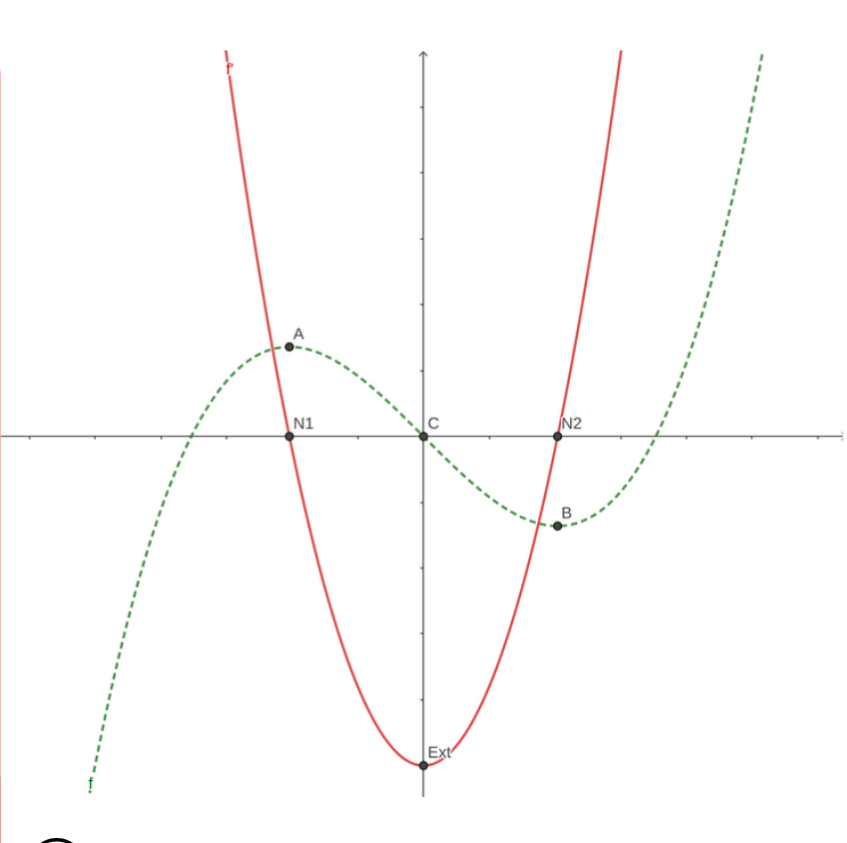
\includegraphics[width=5.5cm]{Bilder/image_Funktionen.png}}
\end{wrapfigure}

Vorgehen beim graphischen Ableiten:
\begin{enumerate}
    \item Stellen mit Steigung 0 suchen, als Nullstellen eintragen
    \item Monoto niebereiche markieren, Funktion in dem Bereich zeichnen
\end{enumerate}
Bei der Rekonstruktion geht man quasi umgekehrt vor
\begin{enumerate}
    \item Nullstellen suchen. Ist die Funktion vor im positiven, dann im negativen Bereiche, dann Hochpunkt eintragen. Andernfalls Tiefpunkt
    \item Extrema suchen, als Wendepunkte eintragen.
    \item Funktion qualitativ zeichnen.
\end{enumerate}

\newpage

\section{Nutzen von der Zweiten Ableitung}

\subsection{Hoch und Tiefpunkte einer Funktion}

Um Herrauszufinden ob Extrema hoch oder Tiefpunkte sind müssen diese in die Zweite Ableitung einfügt werden:

Bei dem Extrema x=6 
\begin{equation}
    f''(x) =6x
\end{equation}
Einsetzen!
\begin{equation}
    f''(6)= 6\cdot 6
\end{equation}
Ausgerechnet:
\begin{equation}
    f''(6)= 36
\end{equation}
36 also > 0 also ein Tiefpunkt

\textbf{Auf vorzeichen Achten!}

\vspace{4mm}


Dann: $f''(x)=6 \cdot 1 \ \Rightarrow 6 > 0 \Rightarrow $ Tiefpunkt

$\Rightarrow$ $f''(x)=6 \cdot (-1) \ \Rightarrow -6 < 0 \Rightarrow$ Hochpunkt

\subsection{Wendepunkte berrechnen}\label{6.2}

Um die Wendepunkte von einer Funktion zu berrechnen:

\begin{enumerate}
    \item Ableitungen Bilden:
    
    $g(x)=-\frac{1}{12}x^4+x^2$
    
    $g'(x)=-\frac{1}{3}x^3+2x$

    $g''(x)=-x^2 + 2$

    $g'''(x)=-2x$

    \item $g''(x)=0$ setzen
    
    $g''(x)=-x^2+2 = 0$

    $\Rightarrow \pm\sqrt{2}$

    \item In die Dritte ableitung setzen:
    
    $g'''(\sqrt{2})=-2 \cdot \sqrt{2}$ $\neq 0$ $\Rightarrow$ WP bei $x = \sqrt{2}$

    $g'''(-\sqrt{2})=-2 \cdot (-\sqrt{2})$ $\neq 0$ $\Rightarrow$ WP bei $x = -\sqrt{2}$

    \item Vollen punkt bestimmen indem man in die Grundform einsetz:
    
    $g(-\sqrt{2})=-\frac{1}{12}(-\sqrt{2})^4+(-\sqrt{2})^2=$  $\frac{5}{3} \ \Rightarrow \ WP(-\sqrt{2} \vert \frac{5}{3}) $

    $g(\sqrt{2})=-\frac{1}{12}(\sqrt{2})^4+(\sqrt{2})^2=$ $\frac{5}{3} \ \Rightarrow \ WP(\sqrt{2} \vert \frac{5}{3}) $



\end{enumerate}

\section{Definitionsmenge}

Die Definitionsmenge ist die Zahl die für X einsetzebar ist.\\
Z.B bei der Funktionen $f(x)= \frac{1}{x}$ kann man keine Null einsetzen.

\subsection{Ganzrationale Formeln}

\begin{itemize}
    \item[$\Rightarrow$] $2x-3$
    \item[$\Rightarrow$] $5x^2-x+2$
    \item[$\Rightarrow$] $x^4-4x^3$
\end{itemize}

Bei Ganzrationale kann man alle Rellen zahlen für das X einfügen also:
$\mathbb{D} = \mathbb{R}$ 
Das $\mathbb{D}$ steht für die Definitionsmenge und $\mathbb{R}$ steht für die Rellenzahlen.


\subsection{Gebrochene rationale Funktionen}

Gebrochene rationale Funktionen also: $f(x)=\frac{1}{x}$

\strich

Gebrochne rationale Funktionen:

Beim beispiel: $f(x)=\frac{x^2}{x^2-4}$ muss man die Nenner gleich 0 setzen!

$x^2 -4 =0$ $\vert \ +4$

$x^\mathbf{2} = 4$ $\vert \ \sqrt[\mathbf{2}]{\ \ }$

Nullstellen:

$x_1 = -2, \  x_2 = 2$

also wäre die Definitionsmenge dann:

$\mathbb{D} = \mathbb{R} \backslash \{ Nullstellen \ des \ Nenners\}$


das $\backslash$ steht für nicht einsetzebar.\\
Und wir nuztzen die Nullstellen, da wenn wir die Nullstellen in die Funktionen im Nenner einsetzen dann kommt da null raus. Und durch null ist nicht teilbar. Also sieht das dann so aus:


$\mathbb{D} = \mathbb{R} \backslash \{-2,2\}$

\subsection{Wurzelfunktionen}

$f(x)=\sqrt{x-3}$

\strich

Innere Funktion $\geq 0$ setzen:

$x-3 \geq 0$ $\vert \ + 3$

$x\geq3$

\strich

$\mathbb{D} = \{ x \ \epsilon \ \mathbb{R} \ \vert \ x \geq3\}$

\subsection{E-Funktionen}
Bsp:
$f(x)=e^x$

\strich

$\mathbb{D} = \mathbb{R}$ 



\newpage

\section{Rekonstruktion}

\subsection{Schlüsselwörter}

Geht durch den Punkt $P(5\vert 3) \ \Rightarrow f(5)=3 $

Schneidet die y-Achse bei 7 $\Rightarrow \ P(0\vert 7) \ \Rightarrow f(0)=7 $

Schneidet die x-Achse bei 2 $\Rightarrow \ P(2\vert 0) \ \Rightarrow f(2)=0 $

\url{https://www.youtube.com/watch?v=xcs3JEWhTGM}


\newpage

\section{Exponentialfunktionen}

%\subsection{Lineares und exponentielles Wachstum}
%
%Linares Wachstum ist Beispielsweise +2 also ein Wachstum das immer gleich bleibt
%
%\hfil \\
%
%Ein exponentielles Wachstum ist ein Wachstum das prozentual ansteigt wodurch sich der Wert 
%vergrößert Beispielsweise: $\cdot$2 oder 2\% 

\subsection{Funktionsgleichung}

\subsubsection{Funktionstypen}

\hspace{\absatz}Wachstumsfunktion $= a > 1$ : $f(x)= 2^{x}$

\hspace{\absatz}Zerfallsfunktion $= 0 < a < 1$ $f(x)=0.2^{x}$

\vspace{\absatz}

\subsubsection{Spiegelung}

Wird der Graph $f(x)=a^{x}$ gespiegelt dann kommt der Graph $g(x)=a^{-x}$ oder $g(x)=(\frac{1}{a})^{x}$

\subsubsection{Streckung}

Um den Graphen zu strecken kommt die Variable \textbf{c} ins Spiel. Dieser Bestimmt die Streckung. Also:
\begin{equation*}
    f(x)=c\cdot a^{x}
\end{equation*}

Oder als Bsp. ein Graphen mit einer Streckung von 2 und einer Steigunsrate von 4: 
\begin{equation*}
    g(x)=2\cdot 4^{x}
\end{equation*}

\subsubsection{Verschiebung in y-Richtung}

Zur Verschiebung in y-Richtung wird die Variable \textbf{b} genutzt:
\begin{equation*}
    f(x)=a^{x}\cdot b
\end{equation*}
Um einen Graphen um 2 in die Y Richtung zu verschieben, wird 2 in b eingesetz
\begin{equation*}
    f(x)=a^{x}\cdot \mathbf{2}
\end{equation*}

\subsubsection{Verschiebung in x-Richtung}

Zur Verschiebung in x-Richtung wird die Variable \textbf{d} genutzt:
\begin{equation*}
    f(x)=a^{x+d}
\end{equation*}
Um einen Graphen um 2 in die X Richtung zu verschieben, wird 2 in d eingesetz
\begin{equation*}
    f(x)=a^{x+\mathbf{2}}
\end{equation*}

\subsubsection{Grundform}

Die Grundform heißt dann:

\begin{equation*}
    f(x)=c\cdot a^{x+d}+b
\end{equation*}


\newpage
\subsection{Bestimmung einer Exponentialfunktion}

\subsubsection{Wurzel}

Ist die Gleichung $x^{4}=8$ löst man mit der 4. Wurzel ($\sqrt[4]{\hspace{2mm}}$). Zum Beispiel:

\vspace{\absatz}

Gegeben: $P(3\vert 5)$ und Gleichung $f(x)=a^{x}$

Wenn der Punkt eingesetz wird kommt dann folgendes raus:

$f(x)=a^x$

$5=a^3 \ \vert \sqrt[3]{\hspace{2mm}}$

$\sqrt[3]{5}\approx 1,71 =a$

\subsubsection{Logarithmus}


\subsection{Halbwertszeit/Verdopplungszeit}

\textbf{Halbwertszeit:} $t_{H}=\log_{a}(0.5)$

\textbf{Verdopplungszeit:} $t_{V}=\log_{a}(2)$











\newpage
\section{Trigonometrische Funktionen}

\subsection{Bogenmaß}

Ein Winkel kann im Grad- oder im \textbf{Bogenmaß} angegeben werden



Im Bogenmaß wird der Winkel $\varphi$  als Verhältnis von Länge des Kreisbogens b zum Radius r definiert.\\
{\Large\begin{math}\varphi = \frac{b}{r}\end{math}}

Die Einheit für die Größe des Winkels ist im Bogenmaß dimensionslos und wird mit Radiant (rad) bezeichnet.
1 rad bezeichnet einen Winkel, bei dem der Bogen gleich lang wie der Radius des Kreises ist.

Für den Einheitskreis mit $r=1$ gilt: \hspace{5mm} $\varphi=b$

Die Größe des Winkel ist gleich der Länge des Bogens

Das kann man sich so vorstellen:

Hier im Bsp. das bei einem Radiant also ungefähr 57,3° der Radius und der Bogen gleich lang ist.
    
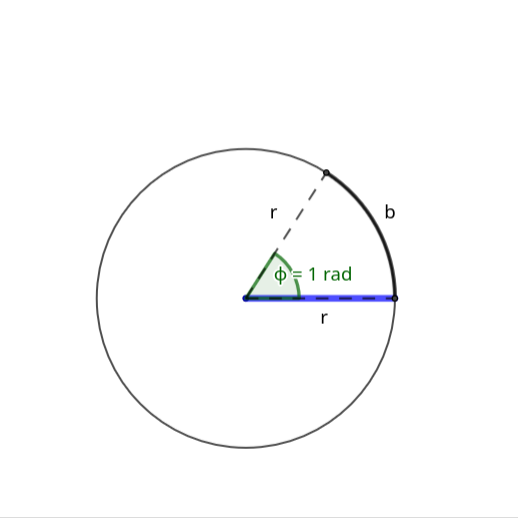
\includegraphics[scale=0.5]{Bilder/Bogenmaß_bsp_2.png}
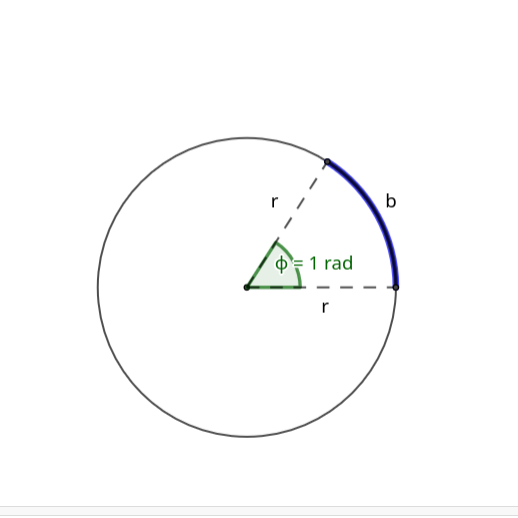
\includegraphics[scale=0.5]{Bilder/Bogenmaß_bsp_1.png}

\subsection{Umrechnung zwischen Grad- und Bogenmaß}

Die Bogenlänge b eines Kreissektors entspricht bei einer ganzen Umdrehung dem Umfang des Kreises und beträgt:
$b=2r\pi$

Also gilt bei einer Vollen Umdrehung:
\begin{equation*}
    \varphi=\frac{b}{r}=\frac{2r\pi}{r}=2\pi
\end{equation*}

Bei einem Winkel von 360° im Gradmaß entspricht ein Wert von $2\pi$ im Bogenmaß.
\textbf{Umrechnung:}
\begin{equation*}
    \alpha(\degree)=\frac{360\degree}{2\pi}\cdot \alpha(\text{in }rad) \text{ bzw. } \alpha(rad)=\frac{2\pi}{360\degree}\cdot \alpha(\text{in }\degree)
\end{equation*}

\subsection{Ableitungen von Trigonometrische Funktionen}

\url{https://simpleclub.com/lessons/mathematik-ableitung-trigonometrischer-funktionen}

\url{https://www.geogebra.org/classroom/ganfmvg9#material/njdn5t8z}






\newpage

\section{Fachwörter}

Monotonieverhalten

\url{https://www.geogebra.org/classroom/e8sbasfy#material/a4s7wueq}

\end{spacing}
\end{document}